\begin{frame}{Challenges of Computer Vision}
\begin{itemize}
    \item Because images are very high-dimensional data, it is difficult for models to capture all possible variety and edge cases included in your data.
    \item Example: When using logistic regression, what happens when you shift an entire image left by one pixel?
\end{itemize}
\end{frame}

\begin{frame}{Challenges of Computer Vision}
\begin{figure}
    \centering
    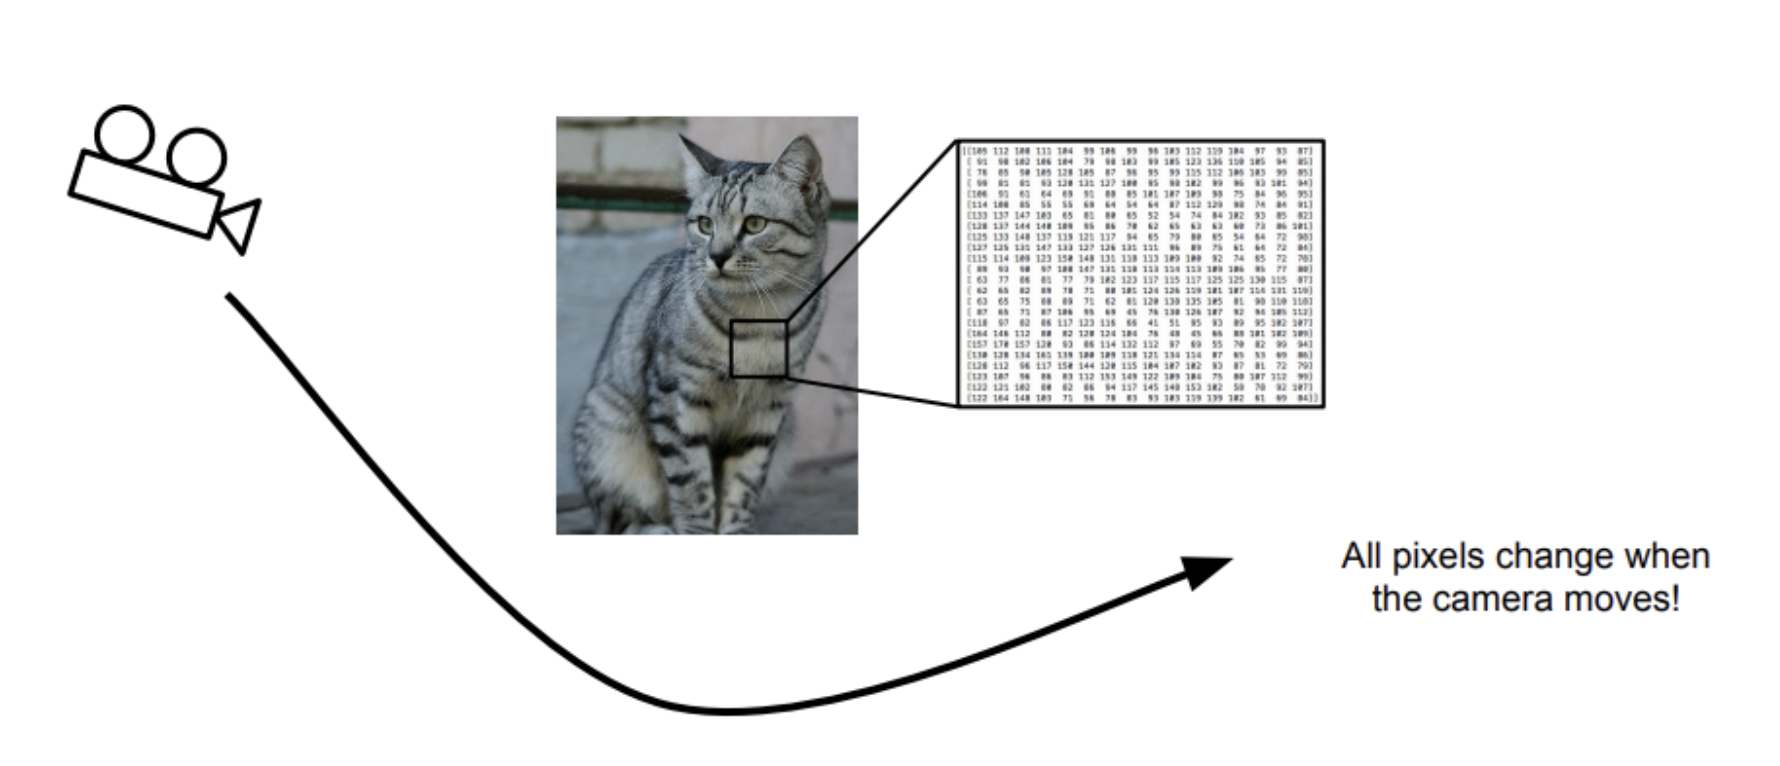
\includegraphics[width=0.9\textwidth]{img/viewpointvariation.png}
    \caption{Viewpoint Variation}
\end{figure}
\footnotetext{http://cs231n.stanford.edu/slides/2019/cs231n\_2019\_lecture02.pdf}
\end{frame}

\begin{frame}{Challenges of Computer Vision}
\begin{figure}
    \centering
    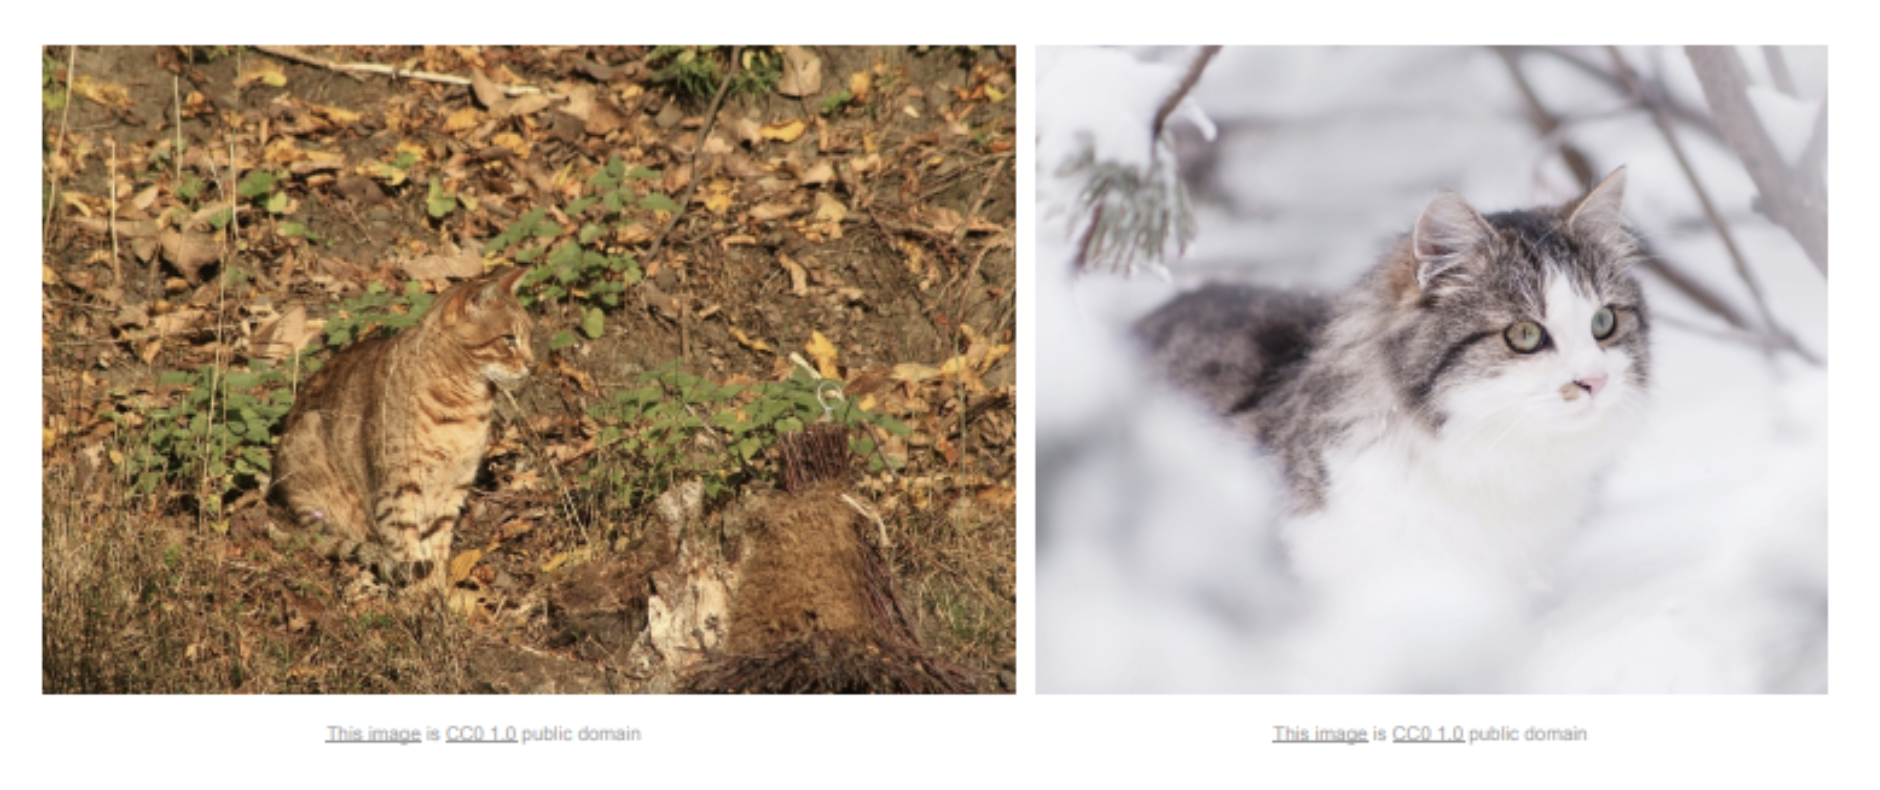
\includegraphics[width=0.9\textwidth]{img/occlusion.png}
    \caption{Background Clutter}
\end{figure}
\footnotetext{http://cs231n.stanford.edu/slides/2019/cs231n\_2019\_lecture02.pdf}
\end{frame}

\begin{frame}{Challenges of Computer Vision}
\begin{figure}
    \centering
    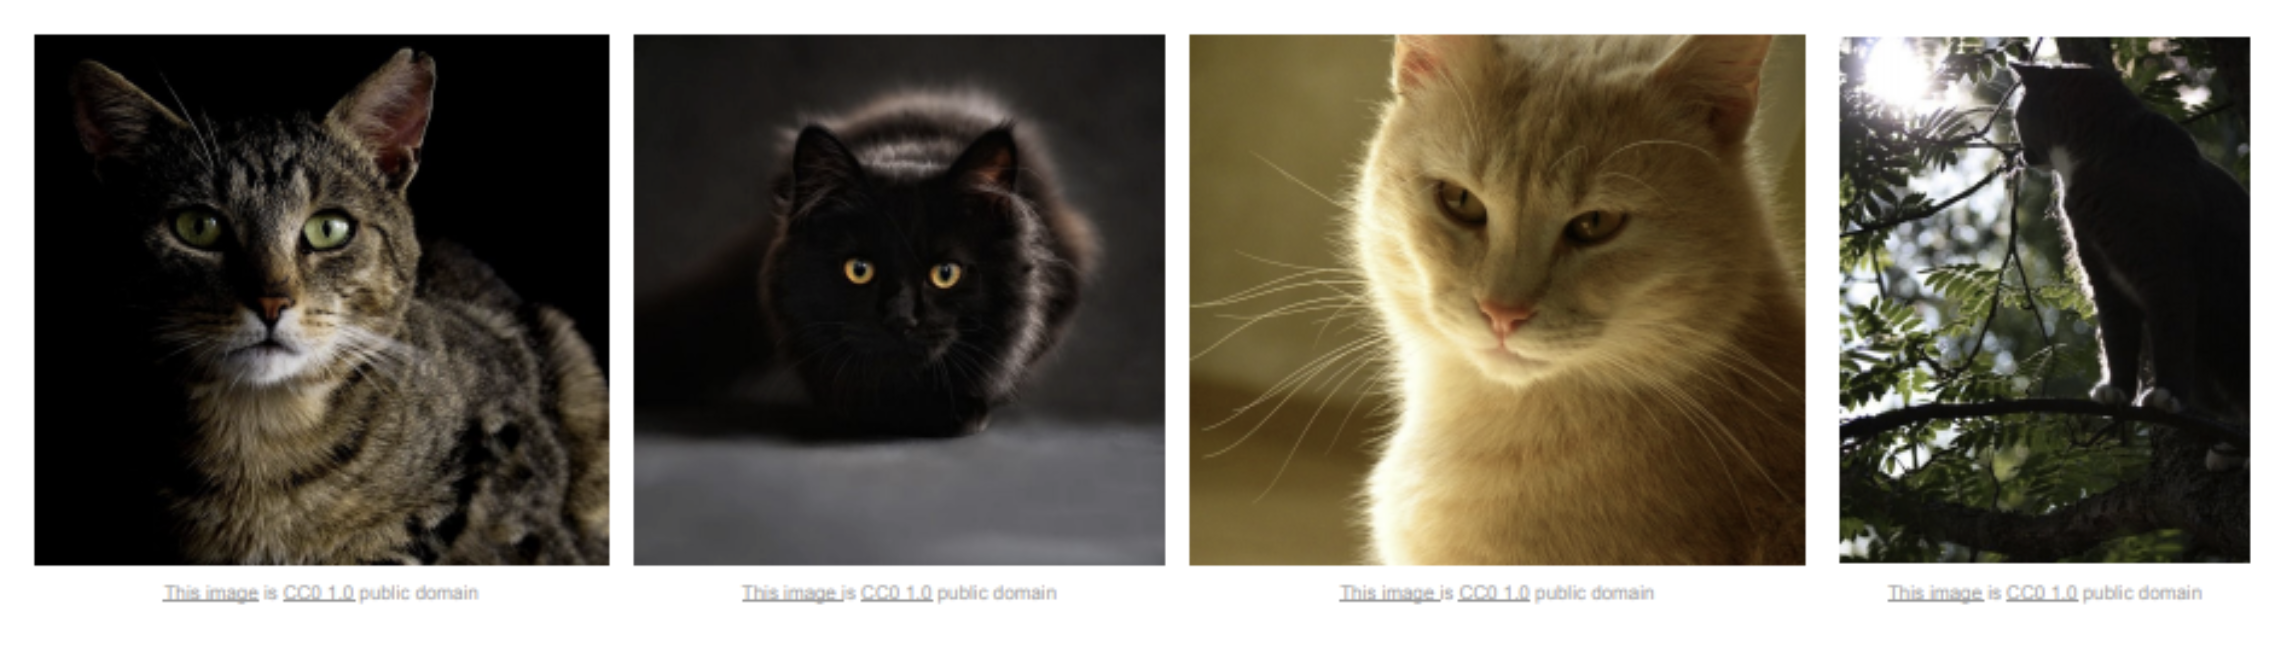
\includegraphics[width=0.9\textwidth]{img/illumination.png}
    \caption{Illumination}
\end{figure}
\footnotetext{http://cs231n.stanford.edu/slides/2019/cs231n\_2019\_lecture02.pdf}
\end{frame}

\begin{frame}{Challenges of Computer Vision}
\begin{figure}
    \centering
    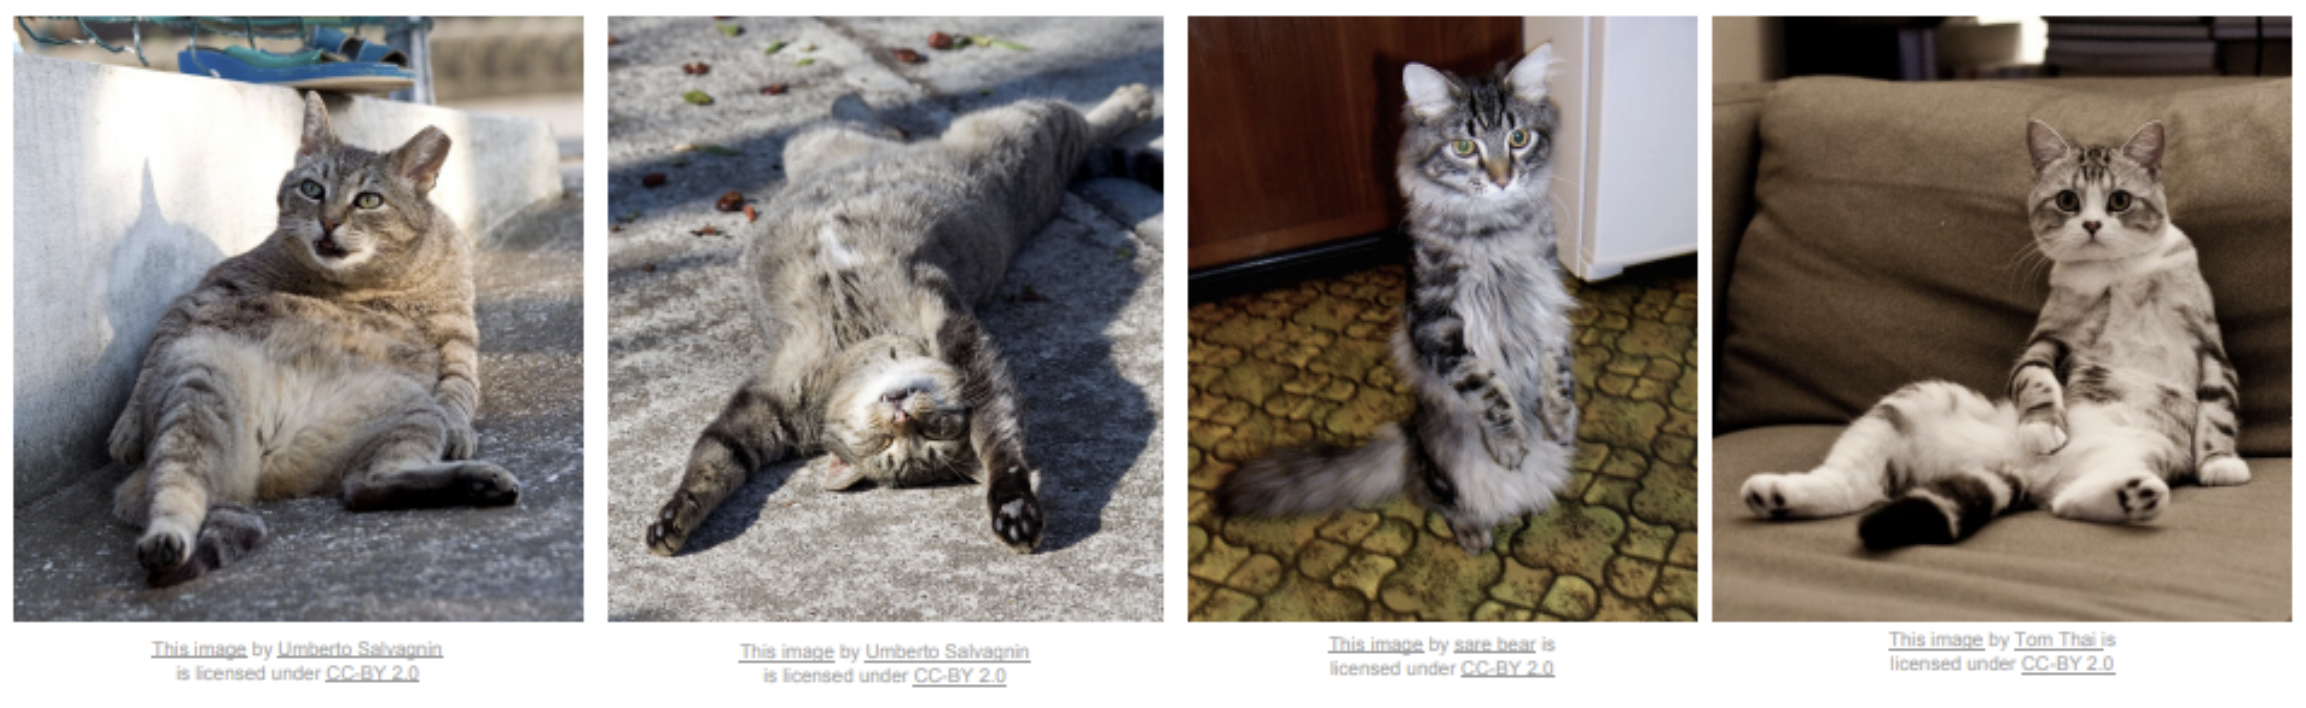
\includegraphics[width=0.9\textwidth]{img/deformation.png}
    \caption{Deformation}
\end{figure}
\footnotetext{http://cs231n.stanford.edu/slides/2019/cs231n\_2019\_lecture02.pdf}
\end{frame}

\begin{frame}{Challenges of Computer Vision}
\begin{figure}
    \centering
    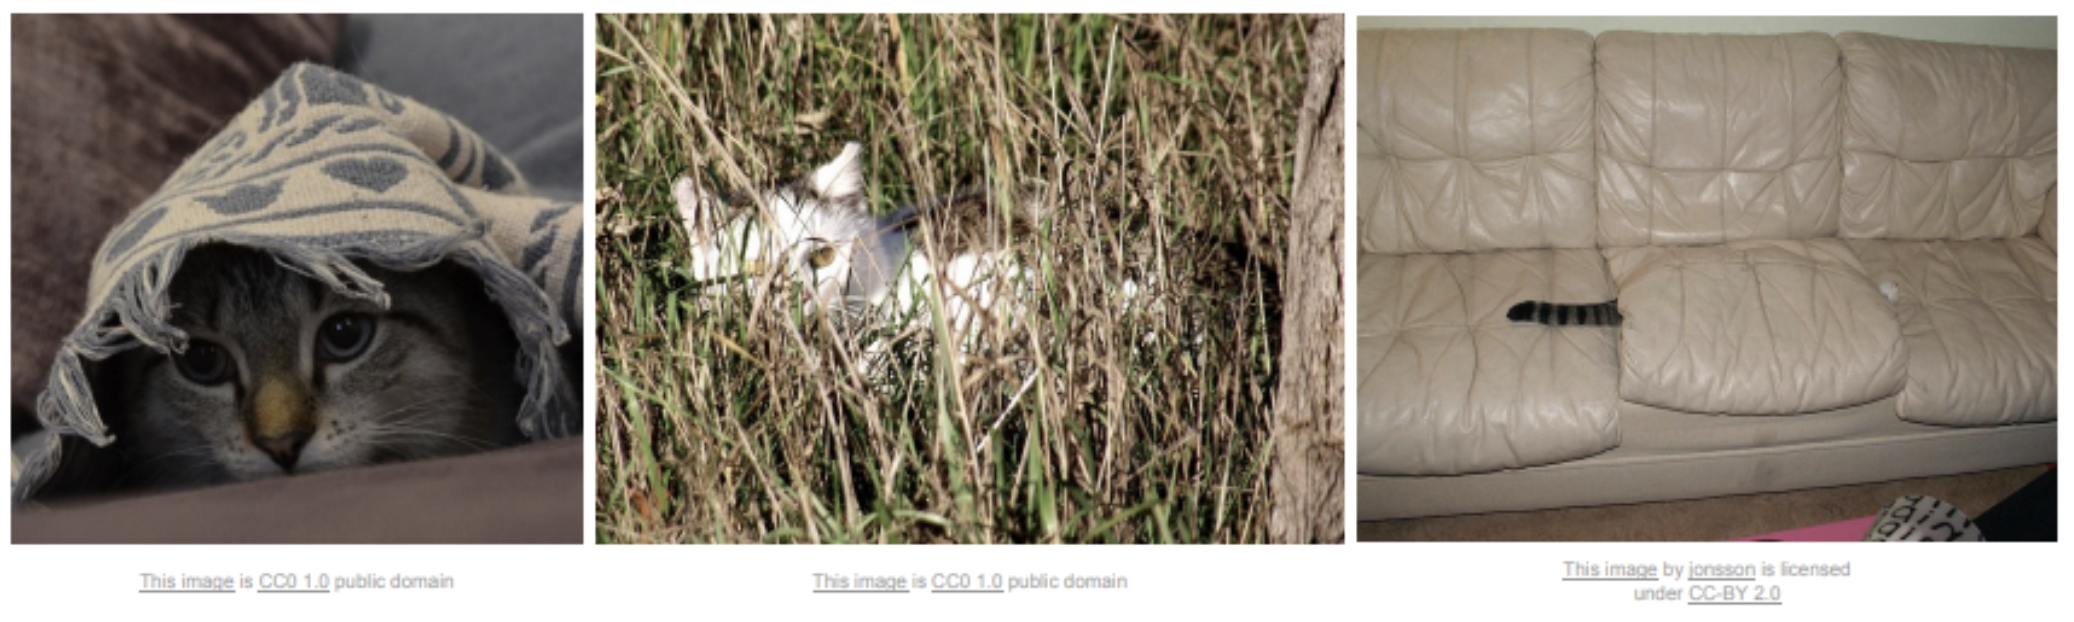
\includegraphics[width=0.9\textwidth]{img/hiding.png}
    \caption{Occlusion}
\end{figure}
\footnotetext{http://cs231n.stanford.edu/slides/2019/cs231n\_2019\_lecture02.pdf}
\end{frame}